\section{理论求解}

\subsection{枚举法}

这里我们假设第一次选择的为第一道门(具有轮换对称性不影响结果),其所有可能结果和最终赢得汽车(用数字 1 表示)的情况如下表所示:

\begin{table}[h]
	\centering
	\begin{tabular}{ccc|cc}
		door 1 & door 2 & door 3 & stick & change \\ \hline
		goat   & goat   & car    & 0     & 1      \\ \hline
		goat   & car    & goat   & 0     & 1      \\ \hline
		car    & goat   & goat   & 1     & 0 
	\end{tabular}
\end{table}

从表中可以看出,改变选择赢得汽车的概率是 $\frac{2}{3}$,而坚持初次选择赢得汽车的概率为 $\frac{1}{3}$。图 \ref{fig:Monty_Tree_Door1} 的树显示了如果玩家最初选择1号门时各种可能结局的可能性。

\begin{figure}[H]
	\centering
	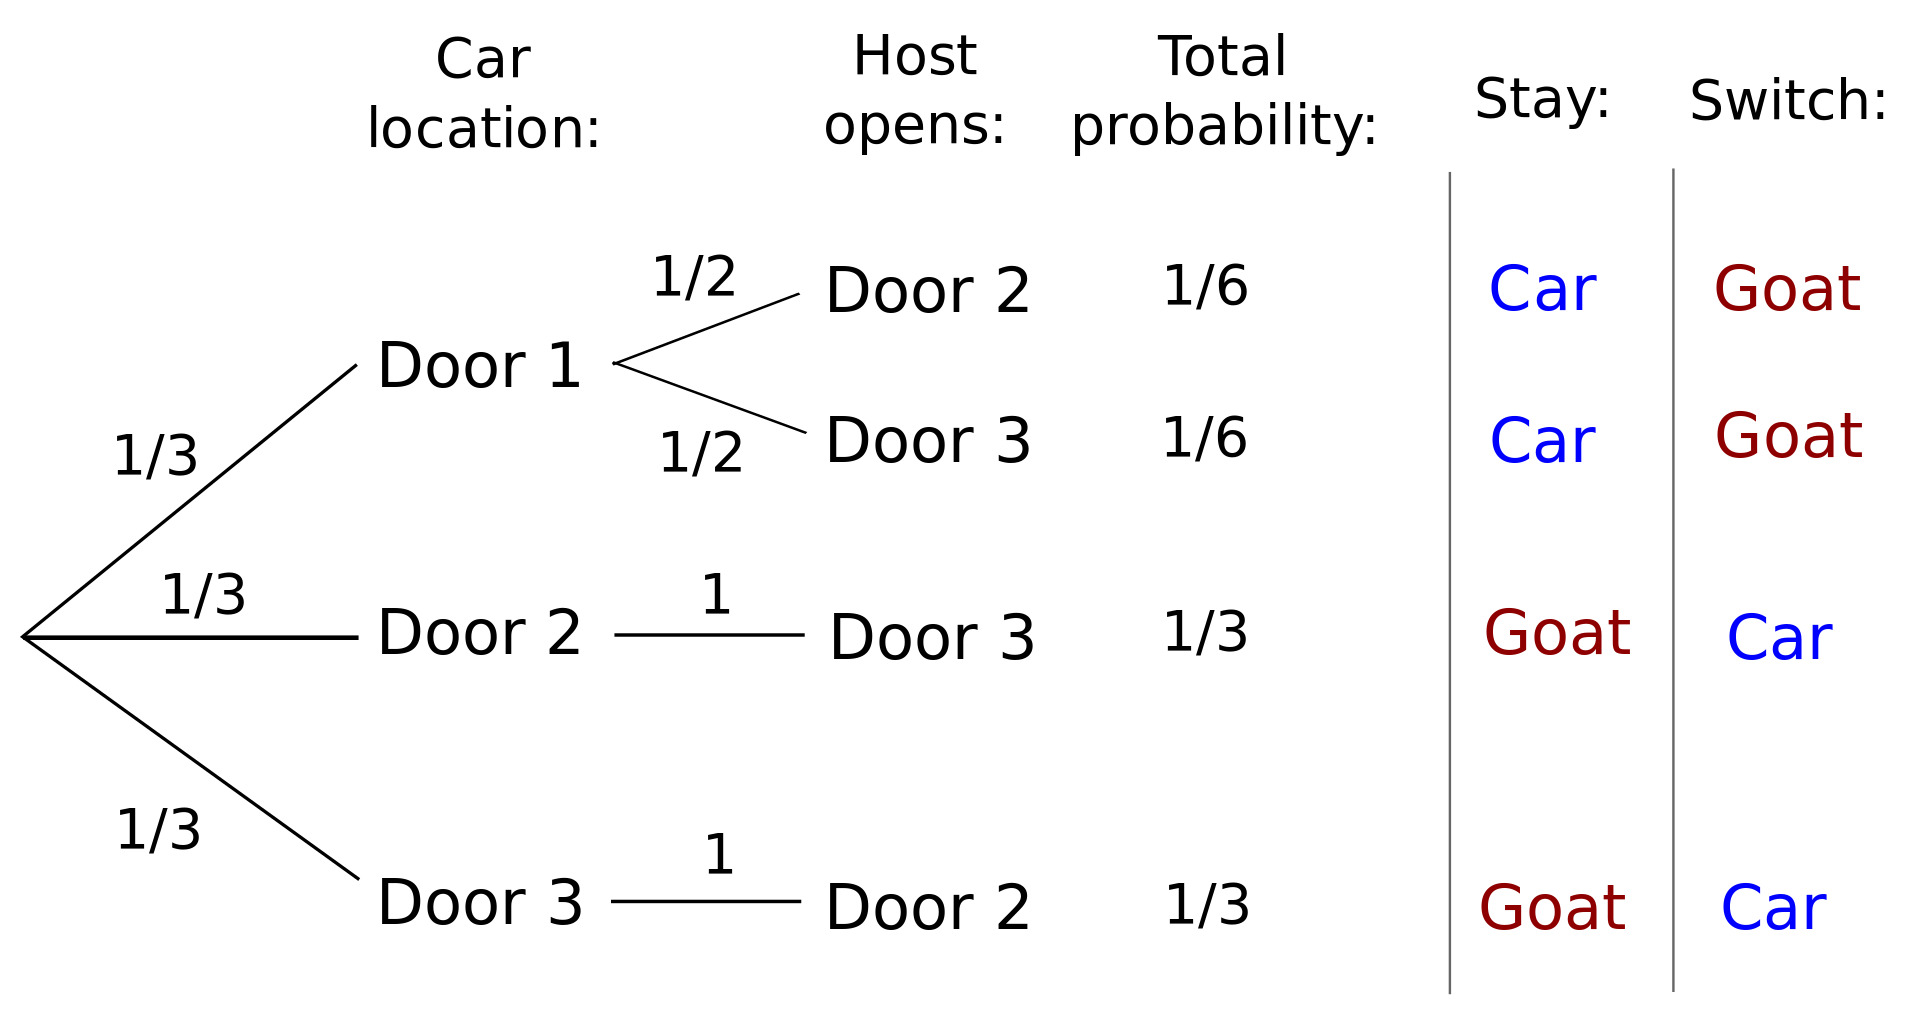
\includegraphics[width=12cm]{figure/tree_door1.jpg}
	\caption{Monty Tree Door1} \label{fig:Monty_Tree_Door1}
\end{figure}

\subsection{概率公式求解}

在上一章中我们给出了两个证明,但其实都包含着同一个错误,即只要主持人选择打开的是含有山羊的门,那么最后得到的结果与主持人打开山羊门的概率无关,即坚持策略获得汽车的概率并非 $P(A_1|B_1C_3)$ 而是 $P(A_1|B_1)$ 或其轮换,改变策略获得汽车的概率并非 $P(A_2|B_1C_3)$ 而是 $P(A_1|B_2)+P(A_1|B_3)$ 或其轮换。

问题的关键在于:主持人知道所有门后面的情况,从而导致了结果违背我们的直觉。

下面给出贝叶斯公式的证明:假设选手选择门 $A$,主持人随后打开 $B$,用 $P(A)$ 表示门 $A$ 后为车,$P(\overline{A})$ 表示 A 后为羊,则选手选择坚持策略获得汽车的概率为 $P(A|\overline{B})$,而选手选择改变策略获得汽车的概率为 $P(\overline{A}|\overline{B})$,下面只计算坚持策略获得汽车概率 $P(A|\overline{B})$,改变策略获得汽车概率为其对立事件,贝叶斯公式如下:

\begin{align*}
P(A|\overline{B})=\frac{P(\overline{B}|A)P(A)}{P(\overline{B}|A)P(A)+P(\overline{B}|\overline{A})P(\overline{A})}
\end{align*}

主持人不会打开有车的门,即 $P(\overline{B}|\overline{A})=1$,另外我们有 $P(A)=\frac{1}{3}$、$P(\overline{A})=\frac{2}{3}$ 和 $P(\overline{B}|A)=1$,代入公式得

\begin{align*}
P(A|\overline{B})=\frac{1\times\frac{1}{3}}{1\times\frac{1}{3}+1\times\frac{2}{3}}=\frac{1}{3}
\end{align*}

故选择坚持策略赢得汽车的概率只有 $\frac{1}{3}$,为了增大概率,应该换门。

假如主持人随意选择一扇门打开,则 $P(\overline{B}|\overline{A})=\frac{1}{2}$,另外我们有 $P(A)=\frac{1}{3}$、$P(\overline{A})=\frac{2}{3}$ 和 $P(\overline{B}|A)=1$,代入公式得

\begin{align*}
P(A|\overline{B})=\frac{1\times\frac{1}{3}}{1\times\frac{1}{3}+\frac{1}{2}\times\frac{2}{3}}=\frac{1}{2}
\end{align*}

可见,如果主持人随机打开一扇门,则换不换门都是一样的概率,因为并没有提供有效信息。

一个更通俗易懂的解释是:当你从三扇门中选择门 A 之后,这扇门后面是车的概率是 $\frac{1}{3}$,门 B 和门 C 有车的概率也是 1/3。但是接下来主持人会给你一个线索。如果奖品在门 B 后面,主持人会打开门 C;如果奖品在门 C 后面,主持人会打开门 B。因此,如果你选择改变策略的话,只要奖品在门 B 或门 C 后你都会赢;但是如果你选择坚持策略,只有奖品在门 A 后你才会赢。

